\documentclass[twoside]{book}

% Packages required by doxygen
\usepackage{fixltx2e}
\usepackage{calc}
\usepackage{doxygen}
\usepackage[export]{adjustbox} % also loads graphicx
\usepackage{graphicx}
\usepackage[utf8]{inputenc}
\usepackage{makeidx}
\usepackage{multicol}
\usepackage{multirow}
\PassOptionsToPackage{warn}{textcomp}
\usepackage{textcomp}
\usepackage[nointegrals]{wasysym}
\usepackage[table]{xcolor}

% Font selection
\usepackage[T1]{fontenc}
\usepackage[scaled=.90]{helvet}
\usepackage{courier}
\usepackage{amssymb}
\usepackage{sectsty}
\renewcommand{\familydefault}{\sfdefault}
\allsectionsfont{%
  \fontseries{bc}\selectfont%
  \color{darkgray}%
}
\renewcommand{\DoxyLabelFont}{%
  \fontseries{bc}\selectfont%
  \color{darkgray}%
}
\newcommand{\+}{\discretionary{\mbox{\scriptsize$\hookleftarrow$}}{}{}}

% Page & text layout
\usepackage{geometry}
\geometry{%
  a4paper,%
  top=2.5cm,%
  bottom=2.5cm,%
  left=2.5cm,%
  right=2.5cm%
}
\tolerance=750
\hfuzz=15pt
\hbadness=750
\setlength{\emergencystretch}{15pt}
\setlength{\parindent}{0cm}
\setlength{\parskip}{3ex plus 2ex minus 2ex}
\makeatletter
\renewcommand{\paragraph}{%
  \@startsection{paragraph}{4}{0ex}{-1.0ex}{1.0ex}{%
    \normalfont\normalsize\bfseries\SS@parafont%
  }%
}
\renewcommand{\subparagraph}{%
  \@startsection{subparagraph}{5}{0ex}{-1.0ex}{1.0ex}{%
    \normalfont\normalsize\bfseries\SS@subparafont%
  }%
}
\makeatother

% Headers & footers
\usepackage{fancyhdr}
\pagestyle{fancyplain}
\fancyhead[LE]{\fancyplain{}{\bfseries\thepage}}
\fancyhead[CE]{\fancyplain{}{}}
\fancyhead[RE]{\fancyplain{}{\bfseries\leftmark}}
\fancyhead[LO]{\fancyplain{}{\bfseries\rightmark}}
\fancyhead[CO]{\fancyplain{}{}}
\fancyhead[RO]{\fancyplain{}{\bfseries\thepage}}
\fancyfoot[LE]{\fancyplain{}{}}
\fancyfoot[CE]{\fancyplain{}{}}
\fancyfoot[RE]{\fancyplain{}{\bfseries\scriptsize Generated by Doxygen }}
\fancyfoot[LO]{\fancyplain{}{\bfseries\scriptsize Generated by Doxygen }}
\fancyfoot[CO]{\fancyplain{}{}}
\fancyfoot[RO]{\fancyplain{}{}}
\renewcommand{\footrulewidth}{0.4pt}
\renewcommand{\chaptermark}[1]{%
  \markboth{#1}{}%
}
\renewcommand{\sectionmark}[1]{%
  \markright{\thesection\ #1}%
}

% Indices & bibliography
\usepackage{natbib}
\usepackage[titles]{tocloft}
\setcounter{tocdepth}{3}
\setcounter{secnumdepth}{5}
\makeindex

% Hyperlinks (required, but should be loaded last)
\usepackage{ifpdf}
\ifpdf
  \usepackage[pdftex,pagebackref=true]{hyperref}
\else
  \usepackage[ps2pdf,pagebackref=true]{hyperref}
\fi
\hypersetup{%
  colorlinks=true,%
  linkcolor=blue,%
  citecolor=blue,%
  unicode%
}

% Custom commands
\newcommand{\clearemptydoublepage}{%
  \newpage{\pagestyle{empty}\cleardoublepage}%
}

\usepackage{caption}
\captionsetup{labelsep=space,justification=centering,font={bf},singlelinecheck=off,skip=4pt,position=top}

%===== C O N T E N T S =====

\begin{document}

% Titlepage & ToC
\hypersetup{pageanchor=false,
             bookmarksnumbered=true,
             pdfencoding=unicode
            }
\pagenumbering{roman}
\begin{titlepage}
\vspace*{7cm}
\begin{center}%
{\Large Concurrent\+Data\+Sharer }\\
\vspace*{1cm}
{\large Generated by Doxygen 1.8.11}\\
\end{center}
\end{titlepage}
\clearemptydoublepage
\tableofcontents
\clearemptydoublepage
\pagenumbering{arabic}
\hypersetup{pageanchor=true}

%--- Begin generated contents ---
\chapter{R\+E\+A\+D\+ME}
\label{md__home_martin_repositories_ConcurrentDataSharer_README}
\hypertarget{md__home_martin_repositories_ConcurrentDataSharer_README}{}
\hyperlink{classConcurrentDataSharer}{Concurrent\+Data\+Sharer} 
\chapter{Hierarchical Index}
\section{Class Hierarchy}
This inheritance list is sorted roughly, but not completely, alphabetically\+:\begin{DoxyCompactList}
\item \contentsline{section}{Blocking\+Queue$<$ T $>$}{\pageref{classBlockingQueue}}{}
\item \contentsline{section}{Blocking\+Queue$<$ Queue\+Element\+Base $\ast$ $>$}{\pageref{classBlockingQueue}}{}
\item \contentsline{section}{client\+Data}{\pageref{classclientData}}{}
\item \contentsline{section}{Concurrent\+Data\+Sharer}{\pageref{classConcurrentDataSharer}}{}
\item \contentsline{section}{Data\+Base\+Element}{\pageref{classDataBaseElement}}{}
\item \contentsline{section}{Queue\+Element\+Base}{\pageref{classQueueElementBase}}{}
\begin{DoxyCompactList}
\item \contentsline{section}{Queue\+Element\+Callback}{\pageref{classQueueElementCallback}}{}
\item \contentsline{section}{Queue\+Element\+Get}{\pageref{classQueueElementGet}}{}
\item \contentsline{section}{Queue\+Element\+Multi\+Send}{\pageref{classQueueElementMultiSend}}{}
\item \contentsline{section}{Queue\+Element\+Set}{\pageref{classQueueElementSet}}{}
\item \contentsline{section}{Queue\+Element\+T\+C\+P\+Send}{\pageref{classQueueElementTCPSend}}{}
\end{DoxyCompactList}
\end{DoxyCompactList}

\chapter{Class Index}
\section{Class List}
Here are the classes, structs, unions and interfaces with brief descriptions\+:\begin{DoxyCompactList}
\item\contentsline{section}{\hyperlink{classBlockingQueue}{Blocking\+Queue$<$ T $>$} \\*\+\_\+\+T\+C\+P\+Send\+Queue = new \hyperlink{classBlockingQueue}{Blocking\+Queue$<$\+Queue\+Element\+Base$\ast$$>$(255)}; \+\_\+\+T\+C\+P\+Send\+Queue-\/$>$put(new Queue\+Element\+Base() ); }{\pageref{classBlockingQueue}}{}
\item\contentsline{section}{\hyperlink{classclientData}{client\+Data} }{\pageref{classclientData}}{}
\item\contentsline{section}{\hyperlink{classConcurrentDataSharer}{Concurrent\+Data\+Sharer} \\*Concurrent\+Data\+Sharer$\ast$ sharer = new \hyperlink{classConcurrentDataSharer}{Concurrent\+Data\+Sharer}(\char`\"{}test\char`\"{}); sharer-\/$>$set$<$int$>$(\char`\"{}data\char`\"{},43); sharer-\/$>$set$<$int$>$(\char`\"{}data1\char`\"{},42); }{\pageref{classConcurrentDataSharer}}{}
\item\contentsline{section}{\hyperlink{classDataBaseElement}{Data\+Base\+Element} }{\pageref{classDataBaseElement}}{}
\item\contentsline{section}{\hyperlink{classQueueElementBase}{Queue\+Element\+Base} }{\pageref{classQueueElementBase}}{}
\item\contentsline{section}{\hyperlink{classQueueElementCallback}{Queue\+Element\+Callback} }{\pageref{classQueueElementCallback}}{}
\item\contentsline{section}{\hyperlink{classQueueElementGet}{Queue\+Element\+Get} }{\pageref{classQueueElementGet}}{}
\item\contentsline{section}{\hyperlink{classQueueElementMultiSend}{Queue\+Element\+Multi\+Send} }{\pageref{classQueueElementMultiSend}}{}
\item\contentsline{section}{\hyperlink{classQueueElementSet}{Queue\+Element\+Set} }{\pageref{classQueueElementSet}}{}
\item\contentsline{section}{\hyperlink{classQueueElementTCPSend}{Queue\+Element\+T\+C\+P\+Send} }{\pageref{classQueueElementTCPSend}}{}
\end{DoxyCompactList}

\chapter{Class Documentation}
\hypertarget{classBlockingQueue}{}\section{Blocking\+Queue$<$ T $>$ Class Template Reference}
\label{classBlockingQueue}\index{Blocking\+Queue$<$ T $>$@{Blocking\+Queue$<$ T $>$}}


\+\_\+\+T\+C\+P\+Send\+Queue = new \hyperlink{classBlockingQueue}{Blocking\+Queue$<$\+Queue\+Element\+Base$\ast$$>$(255)}; \+\_\+\+T\+C\+P\+Send\+Queue-\/$>$put(new Queue\+Element\+Base() );  




{\ttfamily \#include $<$Blocking\+Queue.\+h$>$}

\subsection*{Public Member Functions}
\begin{DoxyCompactItemize}
\item 
\hyperlink{classBlockingQueue_a42f821a61ba22ba27e6d1a434ab27eb2}{Blocking\+Queue} ()
\begin{DoxyCompactList}\small\item\em Constructor. \end{DoxyCompactList}\item 
\hyperlink{classBlockingQueue_adfb84eb73f882a364c8f4cb325b22a1a}{Blocking\+Queue} (std\+::size\+\_\+t capacity)
\begin{DoxyCompactList}\small\item\em Constructor. \end{DoxyCompactList}\item 
void \hyperlink{classBlockingQueue_aeda6a5448ed9b96a56fa1143e6e8ad1c}{Put} (const T \&task)
\begin{DoxyCompactList}\small\item\em put an element in the queue, blocks if full \end{DoxyCompactList}\item 
T \hyperlink{classBlockingQueue_a38dd122eba62f8b5d7ddc1aae266e8da}{Take} ()
\begin{DoxyCompactList}\small\item\em take an element from the queue, blocks if empty \end{DoxyCompactList}\item 
T \hyperlink{classBlockingQueue_a1890f7159b58b97ca1cade42bce9e982}{Front} ()
\begin{DoxyCompactList}\small\item\em returns the front element(been longest in the queue), does not pop, blocks if empty \end{DoxyCompactList}\item 
T \hyperlink{classBlockingQueue_ad2e79734669baee7eeb90e43e9e5d6b9}{Back} ()
\begin{DoxyCompactList}\small\item\em returns the back element(been shortest in the queue), does not pop, blocks if empty \end{DoxyCompactList}\item 
size\+\_\+t \hyperlink{classBlockingQueue_acf02cc9e5671442f6f66c156d9cbe431}{Size} ()
\begin{DoxyCompactList}\small\item\em returns the number of elements in the queue \end{DoxyCompactList}\item 
bool \hyperlink{classBlockingQueue_ae7884eb98569730e5cea0e443d5bb661}{Empty} ()
\begin{DoxyCompactList}\small\item\em returns true if the queue is empty \end{DoxyCompactList}\item 
void \hyperlink{classBlockingQueue_ab3d6fd8cc72986de54213ebdef01245d}{Set\+Capacity} (const size\+\_\+t capacity)
\begin{DoxyCompactList}\small\item\em sets the capacity of the queue \end{DoxyCompactList}\end{DoxyCompactItemize}


\subsection{Detailed Description}
\subsubsection*{template$<$typename T$>$\\*
class Blocking\+Queue$<$ T $>$}

\+\_\+\+T\+C\+P\+Send\+Queue = new \hyperlink{classBlockingQueue}{Blocking\+Queue$<$\+Queue\+Element\+Base$\ast$$>$(255)}; \+\_\+\+T\+C\+P\+Send\+Queue-\/$>$put(new Queue\+Element\+Base() ); 

This is a blocking thread safe F\+I\+FO queue

\begin{DoxyAuthor}{Author}
Martin Soderen
\end{DoxyAuthor}
\begin{DoxyVersion}{Version}
0.\+1
\end{DoxyVersion}
\begin{DoxyDate}{Date}
2017/04/147 00\+:00\+:00
\end{DoxyDate}
Contact\+: \href{mailto:martin.soderen@gmail.com}{\tt martin.\+soderen@gmail.\+com}

Created on\+: Fri Apr 14 00\+:00\+:00 2017

\begin{DoxyParagraph}{Id}

\end{DoxyParagraph}


\subsection{Constructor \& Destructor Documentation}
\index{Blocking\+Queue@{Blocking\+Queue}!Blocking\+Queue@{Blocking\+Queue}}
\index{Blocking\+Queue@{Blocking\+Queue}!Blocking\+Queue@{Blocking\+Queue}}
\subsubsection[{\texorpdfstring{Blocking\+Queue()}{BlockingQueue()}}]{\setlength{\rightskip}{0pt plus 5cm}template$<$typename T$>$ {\bf Blocking\+Queue}$<$ T $>$\+::{\bf Blocking\+Queue} (
\begin{DoxyParamCaption}
{}
\end{DoxyParamCaption}
)\hspace{0.3cm}{\ttfamily [inline]}}\hypertarget{classBlockingQueue_a42f821a61ba22ba27e6d1a434ab27eb2}{}\label{classBlockingQueue_a42f821a61ba22ba27e6d1a434ab27eb2}


Constructor. 


\begin{DoxyParams}{Parameters}
{\em $<$\+T$>$} & template \\
\hline
\end{DoxyParams}
\index{Blocking\+Queue@{Blocking\+Queue}!Blocking\+Queue@{Blocking\+Queue}}
\index{Blocking\+Queue@{Blocking\+Queue}!Blocking\+Queue@{Blocking\+Queue}}
\subsubsection[{\texorpdfstring{Blocking\+Queue(std\+::size\+\_\+t capacity)}{BlockingQueue(std::size_t capacity)}}]{\setlength{\rightskip}{0pt plus 5cm}template$<$typename T$>$ {\bf Blocking\+Queue}$<$ T $>$\+::{\bf Blocking\+Queue} (
\begin{DoxyParamCaption}
\item[{std\+::size\+\_\+t}]{capacity}
\end{DoxyParamCaption}
)\hspace{0.3cm}{\ttfamily [inline]}}\hypertarget{classBlockingQueue_adfb84eb73f882a364c8f4cb325b22a1a}{}\label{classBlockingQueue_adfb84eb73f882a364c8f4cb325b22a1a}


Constructor. 


\begin{DoxyParams}{Parameters}
{\em $<$\+T$>$} & template \\
\hline
{\em capacity} & how many elements you can fill \\
\hline
\end{DoxyParams}


\subsection{Member Function Documentation}
\index{Blocking\+Queue@{Blocking\+Queue}!Back@{Back}}
\index{Back@{Back}!Blocking\+Queue@{Blocking\+Queue}}
\subsubsection[{\texorpdfstring{Back()}{Back()}}]{\setlength{\rightskip}{0pt plus 5cm}template$<$typename T $>$ T {\bf Blocking\+Queue}$<$ T $>$\+::Back (
\begin{DoxyParamCaption}
{}
\end{DoxyParamCaption}
)}\hypertarget{classBlockingQueue_ad2e79734669baee7eeb90e43e9e5d6b9}{}\label{classBlockingQueue_ad2e79734669baee7eeb90e43e9e5d6b9}


returns the back element(been shortest in the queue), does not pop, blocks if empty 

\begin{DoxyReturn}{Returns}
element 
\end{DoxyReturn}
\index{Blocking\+Queue@{Blocking\+Queue}!Empty@{Empty}}
\index{Empty@{Empty}!Blocking\+Queue@{Blocking\+Queue}}
\subsubsection[{\texorpdfstring{Empty()}{Empty()}}]{\setlength{\rightskip}{0pt plus 5cm}template$<$typename T $>$ bool {\bf Blocking\+Queue}$<$ T $>$\+::Empty (
\begin{DoxyParamCaption}
{}
\end{DoxyParamCaption}
)}\hypertarget{classBlockingQueue_ae7884eb98569730e5cea0e443d5bb661}{}\label{classBlockingQueue_ae7884eb98569730e5cea0e443d5bb661}


returns true if the queue is empty 

\begin{DoxyReturn}{Returns}
bool if empty 
\end{DoxyReturn}
\index{Blocking\+Queue@{Blocking\+Queue}!Front@{Front}}
\index{Front@{Front}!Blocking\+Queue@{Blocking\+Queue}}
\subsubsection[{\texorpdfstring{Front()}{Front()}}]{\setlength{\rightskip}{0pt plus 5cm}template$<$typename T $>$ T {\bf Blocking\+Queue}$<$ T $>$\+::Front (
\begin{DoxyParamCaption}
{}
\end{DoxyParamCaption}
)}\hypertarget{classBlockingQueue_a1890f7159b58b97ca1cade42bce9e982}{}\label{classBlockingQueue_a1890f7159b58b97ca1cade42bce9e982}


returns the front element(been longest in the queue), does not pop, blocks if empty 

\begin{DoxyReturn}{Returns}
element 
\end{DoxyReturn}
\index{Blocking\+Queue@{Blocking\+Queue}!Put@{Put}}
\index{Put@{Put}!Blocking\+Queue@{Blocking\+Queue}}
\subsubsection[{\texorpdfstring{Put(const T \&task)}{Put(const T &task)}}]{\setlength{\rightskip}{0pt plus 5cm}template$<$typename T$>$ void {\bf Blocking\+Queue}$<$ T $>$\+::Put (
\begin{DoxyParamCaption}
\item[{const T \&}]{task}
\end{DoxyParamCaption}
)}\hypertarget{classBlockingQueue_aeda6a5448ed9b96a56fa1143e6e8ad1c}{}\label{classBlockingQueue_aeda6a5448ed9b96a56fa1143e6e8ad1c}


put an element in the queue, blocks if full 


\begin{DoxyParams}{Parameters}
{\em task} & element to put in queue \\
\hline
\end{DoxyParams}
\index{Blocking\+Queue@{Blocking\+Queue}!Set\+Capacity@{Set\+Capacity}}
\index{Set\+Capacity@{Set\+Capacity}!Blocking\+Queue@{Blocking\+Queue}}
\subsubsection[{\texorpdfstring{Set\+Capacity(const size\+\_\+t capacity)}{SetCapacity(const size_t capacity)}}]{\setlength{\rightskip}{0pt plus 5cm}template$<$typename T $>$ void {\bf Blocking\+Queue}$<$ T $>$\+::Set\+Capacity (
\begin{DoxyParamCaption}
\item[{const size\+\_\+t}]{capacity}
\end{DoxyParamCaption}
)}\hypertarget{classBlockingQueue_ab3d6fd8cc72986de54213ebdef01245d}{}\label{classBlockingQueue_ab3d6fd8cc72986de54213ebdef01245d}


sets the capacity of the queue 


\begin{DoxyParams}{Parameters}
{\em capacity} & the new capacity of the queue \\
\hline
\end{DoxyParams}
\index{Blocking\+Queue@{Blocking\+Queue}!Size@{Size}}
\index{Size@{Size}!Blocking\+Queue@{Blocking\+Queue}}
\subsubsection[{\texorpdfstring{Size()}{Size()}}]{\setlength{\rightskip}{0pt plus 5cm}template$<$typename T $>$ size\+\_\+t {\bf Blocking\+Queue}$<$ T $>$\+::Size (
\begin{DoxyParamCaption}
{}
\end{DoxyParamCaption}
)}\hypertarget{classBlockingQueue_acf02cc9e5671442f6f66c156d9cbe431}{}\label{classBlockingQueue_acf02cc9e5671442f6f66c156d9cbe431}


returns the number of elements in the queue 

\begin{DoxyReturn}{Returns}
size of queue 
\end{DoxyReturn}
\index{Blocking\+Queue@{Blocking\+Queue}!Take@{Take}}
\index{Take@{Take}!Blocking\+Queue@{Blocking\+Queue}}
\subsubsection[{\texorpdfstring{Take()}{Take()}}]{\setlength{\rightskip}{0pt plus 5cm}template$<$typename T $>$ T {\bf Blocking\+Queue}$<$ T $>$\+::Take (
\begin{DoxyParamCaption}
{}
\end{DoxyParamCaption}
)}\hypertarget{classBlockingQueue_a38dd122eba62f8b5d7ddc1aae266e8da}{}\label{classBlockingQueue_a38dd122eba62f8b5d7ddc1aae266e8da}


take an element from the queue, blocks if empty 

\begin{DoxyReturn}{Returns}
element 
\end{DoxyReturn}


The documentation for this class was generated from the following files\+:\begin{DoxyCompactItemize}
\item 
/home/martin/repositories/\+Concurrent\+Data\+Sharer/include/Blocking\+Queue.\+h\item 
/home/martin/repositories/\+Concurrent\+Data\+Sharer/src/Blocking\+Queue.\+cpp\end{DoxyCompactItemize}

\hypertarget{classclientData}{}\section{client\+Data Class Reference}
\label{classclientData}\index{client\+Data@{client\+Data}}
\subsection*{Public Member Functions}
\begin{DoxyCompactItemize}
\item 
{\bfseries client\+Data} (std\+::string name, std\+::vector$<$ std\+::string $>$ I\+P\+V4, std\+::vector$<$ std\+::string $>$ I\+P\+V6)\hypertarget{classclientData_a975c4515ddc744bc5efa71b6aec38010}{}\label{classclientData_a975c4515ddc744bc5efa71b6aec38010}

\item 
std\+::vector$<$ std\+::string $>$ {\bfseries get\+I\+P\+V4} ()\hypertarget{classclientData_a2f69be4b2b86af0484c0b9111ebc2be0}{}\label{classclientData_a2f69be4b2b86af0484c0b9111ebc2be0}

\item 
std\+::vector$<$ std\+::string $>$ {\bfseries get\+I\+P\+V6} ()\hypertarget{classclientData_a8f9d41274440ddfefbcb450aba9c28d2}{}\label{classclientData_a8f9d41274440ddfefbcb450aba9c28d2}

\item 
std\+::string {\bfseries get\+Name} ()\hypertarget{classclientData_abddedee74c8918168048670cf4104b55}{}\label{classclientData_abddedee74c8918168048670cf4104b55}

\end{DoxyCompactItemize}
\subsection*{Friends}
\begin{DoxyCompactItemize}
\item 
class {\bfseries boost\+::serialization\+::access}\hypertarget{classclientData_ac98d07dd8f7b70e16ccb9a01abf56b9c}{}\label{classclientData_ac98d07dd8f7b70e16ccb9a01abf56b9c}

\end{DoxyCompactItemize}


The documentation for this class was generated from the following file\+:\begin{DoxyCompactItemize}
\item 
/home/martin/repositories/\+Concurrent\+Data\+Sharer/include/structures.\+h\end{DoxyCompactItemize}

\hypertarget{classConcurrentDataSharer}{}\section{Concurrent\+Data\+Sharer Class Reference}
\label{classConcurrentDataSharer}\index{Concurrent\+Data\+Sharer@{Concurrent\+Data\+Sharer}}


Concurrent\+Data\+Sharer$\ast$ sharer = new \hyperlink{classConcurrentDataSharer}{Concurrent\+Data\+Sharer}(\char`\"{}test\char`\"{}); sharer-\/$>$set$<$int$>$(\char`\"{}data\char`\"{},43); sharer-\/$>$set$<$int$>$(\char`\"{}data1\char`\"{},42);.  




{\ttfamily \#include $<$concurrentdatasharer.\+h$>$}

\subsection*{Public Member Functions}
\begin{DoxyCompactItemize}
\item 
\hyperlink{classConcurrentDataSharer_a31adaa38a46a75059bc117aa3b889ead}{Concurrent\+Data\+Sharer} (std\+::string const \&groupname, std\+::string const \&multicastadress=\char`\"{}239.\+255.\+0.\+1\char`\"{}, std\+::string const \&listenadress=\char`\"{}0.\+0.\+0.\+0\char`\"{}, const short multicastport=30001)
\begin{DoxyCompactList}\small\item\em Constructor. \end{DoxyCompactList}\item 
\hyperlink{classConcurrentDataSharer_abfb5ed7099ae718277bdbfeef362c8c9}{$\sim$\+Concurrent\+Data\+Sharer} ()
\begin{DoxyCompactList}\small\item\em Destructor. \end{DoxyCompactList}\item 
{\footnotesize template$<$typename T $>$ }\\void \hyperlink{classConcurrentDataSharer_a61da465e07a98d3b35d5f646d6ebaa33}{set} (std\+::string const \&name, T data)
\begin{DoxyCompactList}\small\item\em Set a local variable, creates it if it does not exists. \end{DoxyCompactList}\item 
{\footnotesize template$<$typename T $>$ }\\T \hyperlink{classConcurrentDataSharer_ab843e7ba2687921eee926d5ec3251ec2}{get} (std\+::string const \&name)
\begin{DoxyCompactList}\small\item\em Get a local variable. \end{DoxyCompactList}\item 
{\footnotesize template$<$typename T $>$ }\\T \hyperlink{classConcurrentDataSharer_a00a171243dde5f2b957f8e338d2fb4cd}{get} (std\+::string const \&client, std\+::string const \&name)
\begin{DoxyCompactList}\small\item\em Get a variable from another client. \end{DoxyCompactList}\item 
std\+::vector$<$ std\+::string $>$ \hyperlink{classConcurrentDataSharer_a10ac5344381b73c61368634efcff7350}{get\+Clients} ()
\begin{DoxyCompactList}\small\item\em to get all connected clients \end{DoxyCompactList}\item 
void \hyperlink{classConcurrentDataSharer_af49ca1b3094d8e5991032aff3e26a39a}{register\+New\+Client\+Callback} (Callback\+Sig func)
\begin{DoxyCompactList}\small\item\em connects a callback when a new clients connects \end{DoxyCompactList}\item 
void \hyperlink{classConcurrentDataSharer_ab1f7d71cb857152ae4c9f5559a3ad32e}{register\+Callback} (std\+::string const \&name, Callback\+Sig func)
\begin{DoxyCompactList}\small\item\em connects a callback if a local variable changes \end{DoxyCompactList}\item 
std\+::string \hyperlink{classConcurrentDataSharer_a7bdc1d74f0d94a9855121f0ddb496bde}{get\+My\+Name} ()
\begin{DoxyCompactList}\small\item\em return the name of this client \end{DoxyCompactList}\item 
std\+::vector$<$ std\+::string $>$ \hyperlink{classConcurrentDataSharer_aba0ce899cc2994d381ab59fb359b8a25}{get\+Client\+Variables} (std\+::string const \&client)
\begin{DoxyCompactList}\small\item\em get a list with the names of a clients variables \end{DoxyCompactList}\end{DoxyCompactItemize}


\subsection{Detailed Description}
Concurrent\+Data\+Sharer$\ast$ sharer = new \hyperlink{classConcurrentDataSharer}{Concurrent\+Data\+Sharer}(\char`\"{}test\char`\"{}); sharer-\/$>$set$<$int$>$(\char`\"{}data\char`\"{},43); sharer-\/$>$set$<$int$>$(\char`\"{}data1\char`\"{},42);. 

This is the main class for the \hyperlink{classConcurrentDataSharer}{Concurrent\+Data\+Sharer}

\begin{DoxyNote}{Note}
This is the shit
\end{DoxyNote}
\begin{DoxyAuthor}{Author}
Martin Soderen
\end{DoxyAuthor}
\begin{DoxyVersion}{Version}
0.\+1
\end{DoxyVersion}
\begin{DoxyDate}{Date}
2017/04/147 00\+:00\+:00
\end{DoxyDate}
Contact\+: \href{mailto:martin.soderen@gmail.com}{\tt martin.\+soderen@gmail.\+com}

Created on\+: Fri Apr 14 00\+:00\+:00 2017

\begin{DoxyParagraph}{Id}

\end{DoxyParagraph}


\subsection{Constructor \& Destructor Documentation}
\index{Concurrent\+Data\+Sharer@{Concurrent\+Data\+Sharer}!Concurrent\+Data\+Sharer@{Concurrent\+Data\+Sharer}}
\index{Concurrent\+Data\+Sharer@{Concurrent\+Data\+Sharer}!Concurrent\+Data\+Sharer@{Concurrent\+Data\+Sharer}}
\subsubsection[{\texorpdfstring{Concurrent\+Data\+Sharer(std\+::string const \&groupname, std\+::string const \&multicastadress=""239.\+255.\+0.\+1"", std\+::string const \&listenadress=""0.\+0.\+0.\+0"", const short multicastport=30001)}{ConcurrentDataSharer(std::string const &groupname, std::string const &multicastadress="239.255.0.1", std::string const &listenadress="0.0.0.0", const short multicastport=30001)}}]{\setlength{\rightskip}{0pt plus 5cm}Concurrent\+Data\+Sharer\+::\+Concurrent\+Data\+Sharer (
\begin{DoxyParamCaption}
\item[{std\+::string const \&}]{groupname, }
\item[{std\+::string const \&}]{multicastadress = {\ttfamily \char`\"{}239.255.0.1\char`\"{}}, }
\item[{std\+::string const \&}]{listenadress = {\ttfamily \char`\"{}0.0.0.0\char`\"{}}, }
\item[{const short}]{multicastport = {\ttfamily 30001}}
\end{DoxyParamCaption}
)}\hypertarget{classConcurrentDataSharer_a31adaa38a46a75059bc117aa3b889ead}{}\label{classConcurrentDataSharer_a31adaa38a46a75059bc117aa3b889ead}


Constructor. 


\begin{DoxyParams}{Parameters}
{\em groupname} & the name for the Concurrent\+Datasharer group to share data with \\
\hline
{\em multicastadress} & the adress for U\+DP broadcasting, default is 239.\+255.\+0.\+1 \\
\hline
{\em listenadress} & the adress for U\+DP broadcasting listening, default is 0.\+0.\+0.\+0 \\
\hline
{\em multicastport} & the port for U\+DP broadcasting, default is 30001 \\
\hline
\end{DoxyParams}
\index{Concurrent\+Data\+Sharer@{Concurrent\+Data\+Sharer}!````~Concurrent\+Data\+Sharer@{$\sim$\+Concurrent\+Data\+Sharer}}
\index{````~Concurrent\+Data\+Sharer@{$\sim$\+Concurrent\+Data\+Sharer}!Concurrent\+Data\+Sharer@{Concurrent\+Data\+Sharer}}
\subsubsection[{\texorpdfstring{$\sim$\+Concurrent\+Data\+Sharer()}{~ConcurrentDataSharer()}}]{\setlength{\rightskip}{0pt plus 5cm}Concurrent\+Data\+Sharer\+::$\sim$\+Concurrent\+Data\+Sharer (
\begin{DoxyParamCaption}
{}
\end{DoxyParamCaption}
)}\hypertarget{classConcurrentDataSharer_abfb5ed7099ae718277bdbfeef362c8c9}{}\label{classConcurrentDataSharer_abfb5ed7099ae718277bdbfeef362c8c9}


Destructor. 

Destructs objects 

\subsection{Member Function Documentation}
\index{Concurrent\+Data\+Sharer@{Concurrent\+Data\+Sharer}!get@{get}}
\index{get@{get}!Concurrent\+Data\+Sharer@{Concurrent\+Data\+Sharer}}
\subsubsection[{\texorpdfstring{get(std\+::string const \&name)}{get(std::string const &name)}}]{\setlength{\rightskip}{0pt plus 5cm}template$<$typename T $>$ T Concurrent\+Data\+Sharer\+::get (
\begin{DoxyParamCaption}
\item[{std\+::string const \&}]{name}
\end{DoxyParamCaption}
)\hspace{0.3cm}{\ttfamily [inline]}}\hypertarget{classConcurrentDataSharer_ab843e7ba2687921eee926d5ec3251ec2}{}\label{classConcurrentDataSharer_ab843e7ba2687921eee926d5ec3251ec2}


Get a local variable. 


\begin{DoxyParams}{Parameters}
{\em name} & the name of the variable \\
\hline
\end{DoxyParams}
\index{Concurrent\+Data\+Sharer@{Concurrent\+Data\+Sharer}!get@{get}}
\index{get@{get}!Concurrent\+Data\+Sharer@{Concurrent\+Data\+Sharer}}
\subsubsection[{\texorpdfstring{get(std\+::string const \&client, std\+::string const \&name)}{get(std::string const &client, std::string const &name)}}]{\setlength{\rightskip}{0pt plus 5cm}template$<$typename T $>$ T Concurrent\+Data\+Sharer\+::get (
\begin{DoxyParamCaption}
\item[{std\+::string const \&}]{client, }
\item[{std\+::string const \&}]{name}
\end{DoxyParamCaption}
)\hspace{0.3cm}{\ttfamily [inline]}}\hypertarget{classConcurrentDataSharer_a00a171243dde5f2b957f8e338d2fb4cd}{}\label{classConcurrentDataSharer_a00a171243dde5f2b957f8e338d2fb4cd}


Get a variable from another client. 


\begin{DoxyParams}{Parameters}
{\em client} & the name of the client \\
\hline
{\em name} & the name of the variable \\
\hline
\end{DoxyParams}
\index{Concurrent\+Data\+Sharer@{Concurrent\+Data\+Sharer}!get\+Clients@{get\+Clients}}
\index{get\+Clients@{get\+Clients}!Concurrent\+Data\+Sharer@{Concurrent\+Data\+Sharer}}
\subsubsection[{\texorpdfstring{get\+Clients()}{getClients()}}]{\setlength{\rightskip}{0pt plus 5cm}std\+::vector$<$ std\+::string $>$ Concurrent\+Data\+Sharer\+::get\+Clients (
\begin{DoxyParamCaption}
{}
\end{DoxyParamCaption}
)}\hypertarget{classConcurrentDataSharer_a10ac5344381b73c61368634efcff7350}{}\label{classConcurrentDataSharer_a10ac5344381b73c61368634efcff7350}


to get all connected clients 

\begin{DoxyReturn}{Returns}
std\+::vector$<$std\+::string$>$ with the names of all the clients 
\end{DoxyReturn}
\index{Concurrent\+Data\+Sharer@{Concurrent\+Data\+Sharer}!get\+Client\+Variables@{get\+Client\+Variables}}
\index{get\+Client\+Variables@{get\+Client\+Variables}!Concurrent\+Data\+Sharer@{Concurrent\+Data\+Sharer}}
\subsubsection[{\texorpdfstring{get\+Client\+Variables(std\+::string const \&client)}{getClientVariables(std::string const &client)}}]{\setlength{\rightskip}{0pt plus 5cm}std\+::vector$<$ std\+::string $>$ Concurrent\+Data\+Sharer\+::get\+Client\+Variables (
\begin{DoxyParamCaption}
\item[{std\+::string const \&}]{client}
\end{DoxyParamCaption}
)}\hypertarget{classConcurrentDataSharer_aba0ce899cc2994d381ab59fb359b8a25}{}\label{classConcurrentDataSharer_aba0ce899cc2994d381ab59fb359b8a25}


get a list with the names of a clients variables 


\begin{DoxyParams}{Parameters}
{\em client} & the name of the client \\
\hline
\end{DoxyParams}
\begin{DoxyReturn}{Returns}
a list with the names of a clients variables 
\end{DoxyReturn}
\index{Concurrent\+Data\+Sharer@{Concurrent\+Data\+Sharer}!get\+My\+Name@{get\+My\+Name}}
\index{get\+My\+Name@{get\+My\+Name}!Concurrent\+Data\+Sharer@{Concurrent\+Data\+Sharer}}
\subsubsection[{\texorpdfstring{get\+My\+Name()}{getMyName()}}]{\setlength{\rightskip}{0pt plus 5cm}std\+::string Concurrent\+Data\+Sharer\+::get\+My\+Name (
\begin{DoxyParamCaption}
{}
\end{DoxyParamCaption}
)\hspace{0.3cm}{\ttfamily [inline]}}\hypertarget{classConcurrentDataSharer_a7bdc1d74f0d94a9855121f0ddb496bde}{}\label{classConcurrentDataSharer_a7bdc1d74f0d94a9855121f0ddb496bde}


return the name of this client 

\begin{DoxyReturn}{Returns}
the name of this client 
\end{DoxyReturn}
\index{Concurrent\+Data\+Sharer@{Concurrent\+Data\+Sharer}!register\+Callback@{register\+Callback}}
\index{register\+Callback@{register\+Callback}!Concurrent\+Data\+Sharer@{Concurrent\+Data\+Sharer}}
\subsubsection[{\texorpdfstring{register\+Callback(std\+::string const \&name, Callback\+Sig func)}{registerCallback(std::string const &name, CallbackSig func)}}]{\setlength{\rightskip}{0pt plus 5cm}void Concurrent\+Data\+Sharer\+::register\+Callback (
\begin{DoxyParamCaption}
\item[{std\+::string const \&}]{name, }
\item[{Callback\+Sig}]{func}
\end{DoxyParamCaption}
)\hspace{0.3cm}{\ttfamily [inline]}}\hypertarget{classConcurrentDataSharer_ab1f7d71cb857152ae4c9f5559a3ad32e}{}\label{classConcurrentDataSharer_ab1f7d71cb857152ae4c9f5559a3ad32e}


connects a callback if a local variable changes 


\begin{DoxyParams}{Parameters}
{\em name} & the name of the variable \\
\hline
{\em func} & the function to connect with change \\
\hline
\end{DoxyParams}
\index{Concurrent\+Data\+Sharer@{Concurrent\+Data\+Sharer}!register\+New\+Client\+Callback@{register\+New\+Client\+Callback}}
\index{register\+New\+Client\+Callback@{register\+New\+Client\+Callback}!Concurrent\+Data\+Sharer@{Concurrent\+Data\+Sharer}}
\subsubsection[{\texorpdfstring{register\+New\+Client\+Callback(\+Callback\+Sig func)}{registerNewClientCallback(CallbackSig func)}}]{\setlength{\rightskip}{0pt plus 5cm}void Concurrent\+Data\+Sharer\+::register\+New\+Client\+Callback (
\begin{DoxyParamCaption}
\item[{Callback\+Sig}]{func}
\end{DoxyParamCaption}
)\hspace{0.3cm}{\ttfamily [inline]}}\hypertarget{classConcurrentDataSharer_af49ca1b3094d8e5991032aff3e26a39a}{}\label{classConcurrentDataSharer_af49ca1b3094d8e5991032aff3e26a39a}


connects a callback when a new clients connects 


\begin{DoxyParams}{Parameters}
{\em func} & the function to connect \\
\hline
\end{DoxyParams}
\index{Concurrent\+Data\+Sharer@{Concurrent\+Data\+Sharer}!set@{set}}
\index{set@{set}!Concurrent\+Data\+Sharer@{Concurrent\+Data\+Sharer}}
\subsubsection[{\texorpdfstring{set(std\+::string const \&name, T data)}{set(std::string const &name, T data)}}]{\setlength{\rightskip}{0pt plus 5cm}template$<$typename T $>$ void Concurrent\+Data\+Sharer\+::set (
\begin{DoxyParamCaption}
\item[{std\+::string const \&}]{name, }
\item[{T}]{data}
\end{DoxyParamCaption}
)\hspace{0.3cm}{\ttfamily [inline]}}\hypertarget{classConcurrentDataSharer_a61da465e07a98d3b35d5f646d6ebaa33}{}\label{classConcurrentDataSharer_a61da465e07a98d3b35d5f646d6ebaa33}


Set a local variable, creates it if it does not exists. 


\begin{DoxyParams}{Parameters}
{\em name} & the name of the variable \\
\hline
{\em data} & the data \\
\hline
\end{DoxyParams}


The documentation for this class was generated from the following files\+:\begin{DoxyCompactItemize}
\item 
/home/martin/repositories/\+Concurrent\+Data\+Sharer/include/concurrentdatasharer.\+h\item 
/home/martin/repositories/\+Concurrent\+Data\+Sharer/src/concurrentdatasharer.\+cpp\end{DoxyCompactItemize}

\hypertarget{classDataBaseElement}{}\section{Data\+Base\+Element Class Reference}
\label{classDataBaseElement}\index{Data\+Base\+Element@{Data\+Base\+Element}}
\subsection*{Public Member Functions}
\begin{DoxyCompactItemize}
\item 
{\bfseries Data\+Base\+Element} (std\+::string const \&, std\+::string const \&)\hypertarget{classDataBaseElement_a253e80879bd04adf40df9d6f1b7828d2}{}\label{classDataBaseElement_a253e80879bd04adf40df9d6f1b7828d2}

\item 
{\bfseries Data\+Base\+Element} (\hyperlink{classQueueElementSet}{Queue\+Element\+Set} $\ast$)\hypertarget{classDataBaseElement_a0e0232a59e6f85e420762f078131279a}{}\label{classDataBaseElement_a0e0232a59e6f85e420762f078131279a}

\item 
std\+::string {\bfseries get\+Data} ()\hypertarget{classDataBaseElement_a2fd512bc7a9f6b1ff64a3bc8f7fdc897}{}\label{classDataBaseElement_a2fd512bc7a9f6b1ff64a3bc8f7fdc897}

\item 
void {\bfseries set\+Data} (std\+::string const \&data)\hypertarget{classDataBaseElement_ae818fb7eec2c99d68c02526de1db08a9}{}\label{classDataBaseElement_ae818fb7eec2c99d68c02526de1db08a9}

\item 
void {\bfseries set\+Callback} (Callback\+Sig func)\hypertarget{classDataBaseElement_a84795ff4c0468accc666c72f22ccc021}{}\label{classDataBaseElement_a84795ff4c0468accc666c72f22ccc021}

\item 
void {\bfseries run\+Callback} ()\hypertarget{classDataBaseElement_a07826cebc0083bd9004e5fbc8cf618b1}{}\label{classDataBaseElement_a07826cebc0083bd9004e5fbc8cf618b1}

\end{DoxyCompactItemize}


The documentation for this class was generated from the following files\+:\begin{DoxyCompactItemize}
\item 
/home/martin/repositories/\+Concurrent\+Data\+Sharer/include/structures.\+h\item 
/home/martin/repositories/\+Concurrent\+Data\+Sharer/src/structures.\+cpp\end{DoxyCompactItemize}

\hypertarget{classQueueElementBase}{}\section{Queue\+Element\+Base Class Reference}
\label{classQueueElementBase}\index{Queue\+Element\+Base@{Queue\+Element\+Base}}


Inheritance diagram for Queue\+Element\+Base\+:\nopagebreak
\begin{figure}[H]
\begin{center}
\leavevmode
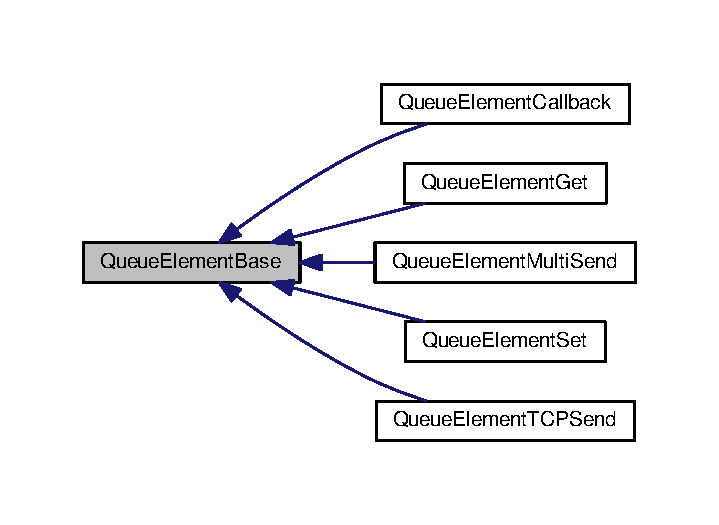
\includegraphics[width=345pt]{classQueueElementBase__inherit__graph}
\end{center}
\end{figure}
\subsection*{Public Member Functions}
\begin{DoxyCompactItemize}
\item 
std\+::string {\bfseries get\+Name} ()\hypertarget{classQueueElementBase_a9c70e7d666436bfeffc430a5346e19a4}{}\label{classQueueElementBase_a9c70e7d666436bfeffc430a5346e19a4}

\item 
std\+::string {\bfseries get\+Data} ()\hypertarget{classQueueElementBase_a10026078f5ea51ffeee0c0de4b0f27c4}{}\label{classQueueElementBase_a10026078f5ea51ffeee0c0de4b0f27c4}

\end{DoxyCompactItemize}
\subsection*{Protected Attributes}
\begin{DoxyCompactItemize}
\item 
std\+::string {\bfseries \+\_\+name}\hypertarget{classQueueElementBase_a0d3714c99af515977f595be0f643d41a}{}\label{classQueueElementBase_a0d3714c99af515977f595be0f643d41a}

\item 
std\+::string {\bfseries \+\_\+data}\hypertarget{classQueueElementBase_a7cb39ad6820aadc40656013e48955833}{}\label{classQueueElementBase_a7cb39ad6820aadc40656013e48955833}

\end{DoxyCompactItemize}


The documentation for this class was generated from the following files\+:\begin{DoxyCompactItemize}
\item 
/home/martin/repositories/\+Concurrent\+Data\+Sharer/include/structures.\+h\item 
/home/martin/repositories/\+Concurrent\+Data\+Sharer/src/structures.\+cpp\end{DoxyCompactItemize}

\hypertarget{classQueueElementCallback}{}\section{Queue\+Element\+Callback Class Reference}
\label{classQueueElementCallback}\index{Queue\+Element\+Callback@{Queue\+Element\+Callback}}


Inheritance diagram for Queue\+Element\+Callback\+:\nopagebreak
\begin{figure}[H]
\begin{center}
\leavevmode
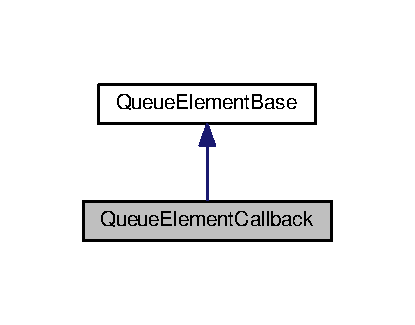
\includegraphics[width=199pt]{classQueueElementCallback__inherit__graph}
\end{center}
\end{figure}


Collaboration diagram for Queue\+Element\+Callback\+:\nopagebreak
\begin{figure}[H]
\begin{center}
\leavevmode
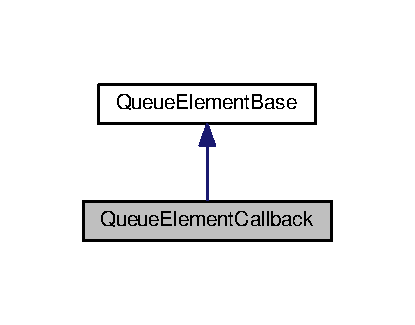
\includegraphics[width=199pt]{classQueueElementCallback__coll__graph}
\end{center}
\end{figure}
\subsection*{Public Member Functions}
\begin{DoxyCompactItemize}
\item 
{\bfseries Queue\+Element\+Callback} (std\+::string const \&name, Callback\+Sig func)\hypertarget{classQueueElementCallback_ac8dfce454a7807e007a00235db8f24ec}{}\label{classQueueElementCallback_ac8dfce454a7807e007a00235db8f24ec}

\item 
Callback\+Sig {\bfseries get\+Callback} ()\hypertarget{classQueueElementCallback_a4b48898ed348624818f064f7dbd75a73}{}\label{classQueueElementCallback_a4b48898ed348624818f064f7dbd75a73}

\end{DoxyCompactItemize}
\subsection*{Additional Inherited Members}


The documentation for this class was generated from the following file\+:\begin{DoxyCompactItemize}
\item 
/home/martin/repositories/\+Concurrent\+Data\+Sharer/include/structures.\+h\end{DoxyCompactItemize}

\hypertarget{classQueueElementGet}{}\section{Queue\+Element\+Get Class Reference}
\label{classQueueElementGet}\index{Queue\+Element\+Get@{Queue\+Element\+Get}}


Inheritance diagram for Queue\+Element\+Get\+:\nopagebreak
\begin{figure}[H]
\begin{center}
\leavevmode
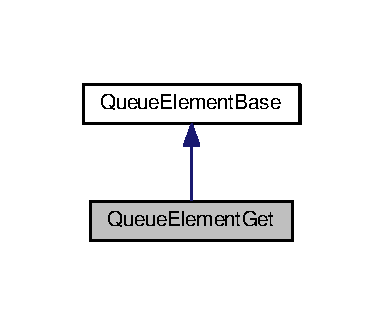
\includegraphics[width=184pt]{classQueueElementGet__inherit__graph}
\end{center}
\end{figure}


Collaboration diagram for Queue\+Element\+Get\+:\nopagebreak
\begin{figure}[H]
\begin{center}
\leavevmode
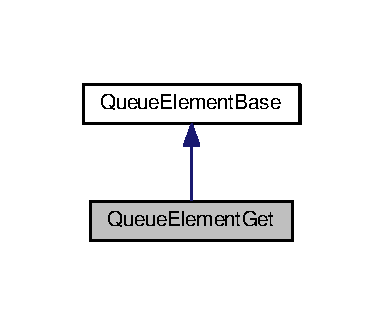
\includegraphics[width=184pt]{classQueueElementGet__coll__graph}
\end{center}
\end{figure}
\subsection*{Public Member Functions}
\begin{DoxyCompactItemize}
\item 
{\bfseries Queue\+Element\+Get} (std\+::string const \&)\hypertarget{classQueueElementGet_a45a2f0b71296d26da6934accf0b2dd16}{}\label{classQueueElementGet_a45a2f0b71296d26da6934accf0b2dd16}

\item 
std\+::string {\bfseries get\+Data} ()\hypertarget{classQueueElementGet_a6a0d5bc87f2f06ec8f31ca4f1ef249a1}{}\label{classQueueElementGet_a6a0d5bc87f2f06ec8f31ca4f1ef249a1}

\item 
void {\bfseries set\+Data} (std\+::string const \&)\hypertarget{classQueueElementGet_aefa414c7a54bf6db99e201b887710061}{}\label{classQueueElementGet_aefa414c7a54bf6db99e201b887710061}

\end{DoxyCompactItemize}
\subsection*{Additional Inherited Members}


The documentation for this class was generated from the following files\+:\begin{DoxyCompactItemize}
\item 
/home/martin/repositories/\+Concurrent\+Data\+Sharer/include/structures.\+h\item 
/home/martin/repositories/\+Concurrent\+Data\+Sharer/src/structures.\+cpp\end{DoxyCompactItemize}

\hypertarget{classQueueElementMultiSend}{}\section{Queue\+Element\+Multi\+Send Class Reference}
\label{classQueueElementMultiSend}\index{Queue\+Element\+Multi\+Send@{Queue\+Element\+Multi\+Send}}


Inheritance diagram for Queue\+Element\+Multi\+Send\+:\nopagebreak
\begin{figure}[H]
\begin{center}
\leavevmode
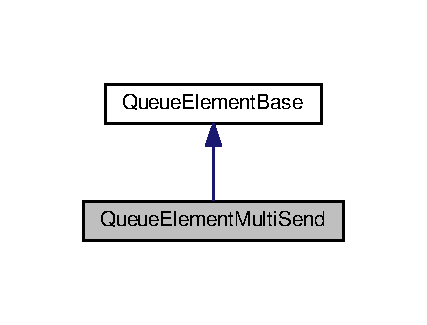
\includegraphics[width=205pt]{classQueueElementMultiSend__inherit__graph}
\end{center}
\end{figure}


Collaboration diagram for Queue\+Element\+Multi\+Send\+:\nopagebreak
\begin{figure}[H]
\begin{center}
\leavevmode
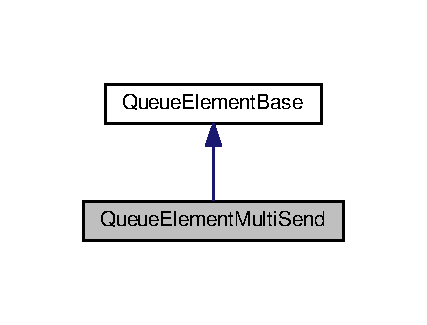
\includegraphics[width=205pt]{classQueueElementMultiSend__coll__graph}
\end{center}
\end{figure}
\subsection*{Public Member Functions}
\begin{DoxyCompactItemize}
\item 
{\bfseries Queue\+Element\+Multi\+Send} (std\+::string const \&, std\+::string const \&, Multi\+Send)\hypertarget{classQueueElementMultiSend_a07b95e3ae8badfb17d67f8e0714c3667}{}\label{classQueueElementMultiSend_a07b95e3ae8badfb17d67f8e0714c3667}

\item 
Multi\+Send {\bfseries get\+Purpose} ()\hypertarget{classQueueElementMultiSend_a2318835ba88e5020022365640a50281b}{}\label{classQueueElementMultiSend_a2318835ba88e5020022365640a50281b}

\end{DoxyCompactItemize}
\subsection*{Friends}
\begin{DoxyCompactItemize}
\item 
class {\bfseries boost\+::serialization\+::access}\hypertarget{classQueueElementMultiSend_ac98d07dd8f7b70e16ccb9a01abf56b9c}{}\label{classQueueElementMultiSend_ac98d07dd8f7b70e16ccb9a01abf56b9c}

\end{DoxyCompactItemize}
\subsection*{Additional Inherited Members}


The documentation for this class was generated from the following files\+:\begin{DoxyCompactItemize}
\item 
/home/martin/repositories/\+Concurrent\+Data\+Sharer/include/structures.\+h\item 
/home/martin/repositories/\+Concurrent\+Data\+Sharer/src/structures.\+cpp\end{DoxyCompactItemize}

\hypertarget{classQueueElementSet}{}\section{Queue\+Element\+Set Class Reference}
\label{classQueueElementSet}\index{Queue\+Element\+Set@{Queue\+Element\+Set}}


Inheritance diagram for Queue\+Element\+Set\+:\nopagebreak
\begin{figure}[H]
\begin{center}
\leavevmode
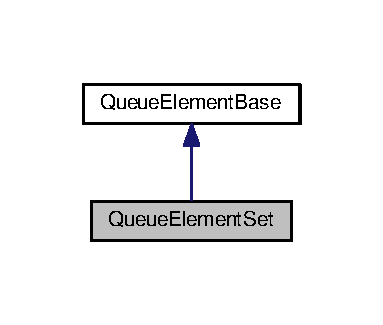
\includegraphics[width=184pt]{classQueueElementSet__inherit__graph}
\end{center}
\end{figure}


Collaboration diagram for Queue\+Element\+Set\+:\nopagebreak
\begin{figure}[H]
\begin{center}
\leavevmode
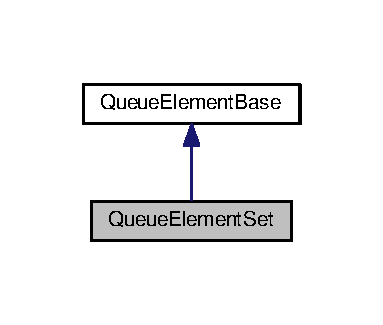
\includegraphics[width=184pt]{classQueueElementSet__coll__graph}
\end{center}
\end{figure}
\subsection*{Public Member Functions}
\begin{DoxyCompactItemize}
\item 
{\bfseries Queue\+Element\+Set} (std\+::string const \&, std\+::string const \&)\hypertarget{classQueueElementSet_a3d61532cdffb0f520a4080c925416dd0}{}\label{classQueueElementSet_a3d61532cdffb0f520a4080c925416dd0}

\end{DoxyCompactItemize}
\subsection*{Additional Inherited Members}


The documentation for this class was generated from the following files\+:\begin{DoxyCompactItemize}
\item 
/home/martin/repositories/\+Concurrent\+Data\+Sharer/include/structures.\+h\item 
/home/martin/repositories/\+Concurrent\+Data\+Sharer/src/structures.\+cpp\end{DoxyCompactItemize}

\hypertarget{classQueueElementTCPSend}{}\section{Queue\+Element\+T\+C\+P\+Send Class Reference}
\label{classQueueElementTCPSend}\index{Queue\+Element\+T\+C\+P\+Send@{Queue\+Element\+T\+C\+P\+Send}}


Inheritance diagram for Queue\+Element\+T\+C\+P\+Send\+:\nopagebreak
\begin{figure}[H]
\begin{center}
\leavevmode
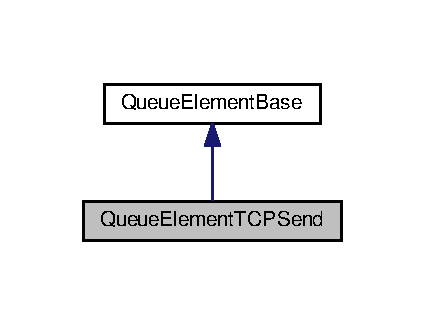
\includegraphics[width=204pt]{classQueueElementTCPSend__inherit__graph}
\end{center}
\end{figure}


Collaboration diagram for Queue\+Element\+T\+C\+P\+Send\+:\nopagebreak
\begin{figure}[H]
\begin{center}
\leavevmode
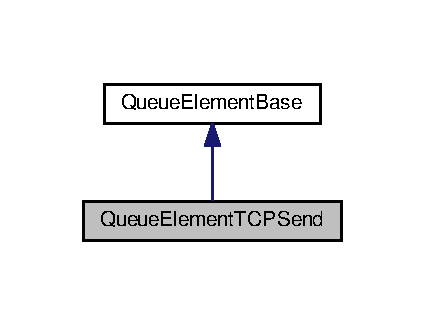
\includegraphics[width=204pt]{classQueueElementTCPSend__coll__graph}
\end{center}
\end{figure}
\subsection*{Public Member Functions}
\begin{DoxyCompactItemize}
\item 
{\bfseries Queue\+Element\+T\+C\+P\+Send} (std\+::string const \&name, std\+::string const \&data, T\+C\+P\+Send purpose, bool respons)\hypertarget{classQueueElementTCPSend_a3aa9f7c8e3173d2864360e141d860fab}{}\label{classQueueElementTCPSend_a3aa9f7c8e3173d2864360e141d860fab}

\item 
void {\bfseries set\+Tag} (std\+::string const \&tag)\hypertarget{classQueueElementTCPSend_a198be59bc4f6f914c85027211fcb8aa1}{}\label{classQueueElementTCPSend_a198be59bc4f6f914c85027211fcb8aa1}

\item 
std\+::string {\bfseries get\+Tag} ()\hypertarget{classQueueElementTCPSend_a4383f6077d21932f6dead51d8a49f30d}{}\label{classQueueElementTCPSend_a4383f6077d21932f6dead51d8a49f30d}

\item 
bool {\bfseries get\+Respons\+Required} ()\hypertarget{classQueueElementTCPSend_a01857057cc95486764d996723a4a2f5e}{}\label{classQueueElementTCPSend_a01857057cc95486764d996723a4a2f5e}

\item 
T\+C\+P\+Send {\bfseries get\+Purpose} ()\hypertarget{classQueueElementTCPSend_a7a42ab6be9a3811c7eaee728b41c3754}{}\label{classQueueElementTCPSend_a7a42ab6be9a3811c7eaee728b41c3754}

\item 
void {\bfseries set\+Requestor} (std\+::string const \&requestor)\hypertarget{classQueueElementTCPSend_a788d2b6a8667c99a5d7282e65124c642}{}\label{classQueueElementTCPSend_a788d2b6a8667c99a5d7282e65124c642}

\item 
std\+::string {\bfseries get\+Requestor} ()\hypertarget{classQueueElementTCPSend_a4d75205d089624600e851ea7745caa16}{}\label{classQueueElementTCPSend_a4d75205d089624600e851ea7745caa16}

\item 
void {\bfseries set\+Data} (std\+::string const \&data)\hypertarget{classQueueElementTCPSend_aaa0e006f646046245095aa28b1cb2e98}{}\label{classQueueElementTCPSend_aaa0e006f646046245095aa28b1cb2e98}

\item 
std\+::string {\bfseries get\+Data} ()\hypertarget{classQueueElementTCPSend_a5537c19f909690c8aff22506d634af97}{}\label{classQueueElementTCPSend_a5537c19f909690c8aff22506d634af97}

\item 
std\+::string {\bfseries get\+Data\+None\+Blocking} ()\hypertarget{classQueueElementTCPSend_a37ff81fd3e511fb704478da714024f00}{}\label{classQueueElementTCPSend_a37ff81fd3e511fb704478da714024f00}

\end{DoxyCompactItemize}
\subsection*{Friends}
\begin{DoxyCompactItemize}
\item 
class {\bfseries boost\+::serialization\+::access}\hypertarget{classQueueElementTCPSend_ac98d07dd8f7b70e16ccb9a01abf56b9c}{}\label{classQueueElementTCPSend_ac98d07dd8f7b70e16ccb9a01abf56b9c}

\end{DoxyCompactItemize}
\subsection*{Additional Inherited Members}


The documentation for this class was generated from the following file\+:\begin{DoxyCompactItemize}
\item 
/home/martin/repositories/\+Concurrent\+Data\+Sharer/include/structures.\+h\end{DoxyCompactItemize}

%--- End generated contents ---

% Index
\backmatter
\newpage
\phantomsection
\clearemptydoublepage
\addcontentsline{toc}{chapter}{Index}
\printindex

\end{document}
